\documentclass[a4paper, 14pt]{extarticle}
\usepackage[english,russian]{babel}
\usepackage[T1]{fontenc}
\usepackage[utf8]{inputenc}
\usepackage{fontspec}
\usepackage{indentfirst}
\usepackage{enumitem}
\usepackage{graphicx}
\usepackage[
  left=30mm,
  right=10mm,
  top=20mm,
  bottom=20mm
]{geometry}
\usepackage{parskip}
\usepackage{titlesec}
\usepackage{xurl}
\usepackage{hyperref}
\usepackage{float}
\usepackage[
  figurename=Рисунок,
  labelsep=endash,
  justification=centering
]{caption}
\usepackage[outputdir=build, newfloat]{minted}
\usepackage{chngcntr}

\selectlanguage{russian}

\hypersetup{
  colorlinks=true,
  linkcolor=black,
  filecolor=blue,
  urlcolor=blue,
}

\renewcommand*{\labelitemi}{---}
\setmainfont{Times New Roman}
\setmonofont{JetBrains Mono}[
  SizeFeatures={Size=11},
]

\newenvironment{code}{\captionsetup{type=figure}}{}
\BeforeBeginEnvironment{code}{\bigskip}
\AfterEndEnvironment{code}{\bigskip}

\setminted{
  fontsize=\footnotesize,
}

\setlength{\parskip}{6pt}

\setlength{\parindent}{1.25cm}
\setlist[itemize]{itemsep=0em,topsep=0em,parsep=0em,partopsep=0em,leftmargin=2.0cm,wide}
\setlist[enumerate]{itemsep=0em,topsep=0em,parsep=0em,partopsep=0em,leftmargin=2.0cm,wide}

\renewcommand{\thesection}{\indent\arabic{section}.}
\renewcommand{\thesubsection}{\indent\thesection\arabic{subsection}.}
\renewcommand{\thesubsubsection}{\indent\thesubsection\arabic{subsubsection}.}

\titleformat{\section}{\normalfont\bfseries}{\thesection}{0.5em}{}
\titleformat{\subsection}{\normalfont\bfseries}{\thesubsection}{0.5em}{}
\titleformat{\subsubsection}{\normalfont\bfseries}{\thesubsubsection}{0.5em}{}

\titleformat*{\section}{\normalfont\bfseries}
\titleformat*{\subsection}{\normalfont\bfseries}
\titleformat*{\subsubsection}{\normalfont\bfseries}

\titlespacing{\section}{\parindent}{\parskip}{\parskip}
\titlespacing{\subsection}{\parindent}{\parskip}{\parskip}
\titlespacing{\subsubsection}{\parindent}{\parskip}{\parskip}

\begin{document}

\begin{titlepage}
  \vspace{0pt plus2fill}
  \noindent

  \vspace{0pt plus6fill}
  \begin{center}
    {
    \bfseries
    Министерство науки и высшего образования Российской Федерации
    {
    \scriptsize
    ФЕДЕРАЛЬНОЕ ГОСУДАРСТВЕННОЕ АВТОНОМНОЕ ОБРАЗОВАТЕЛЬНОЕ УЧРЕЖДЕНИЕ ВЫСШЕГО
    ОБРАЗОВАНИЯ
    }
    «Национальный исследовательский университет ИТМО»

    (Университет ИТМО)

    \begin{minipage}[t]{0.42\textwidth}
      \vspace*{0pt}
      \begin{flushright}
        Факультет

        Образовательная программа
      \end{flushright}
    \end{minipage}
    \begin{minipage}[t]{0.57\textwidth}
      \vspace*{0pt}
      \begin{flushright}
        Инфокоммуникационных технологий

        11.03.02 Программирование в инфокоммуникационных системах
      \end{flushright}
    \end{minipage}
    }

    \vspace{0pt plus5fill}

    \LARGE{
      ОТЧЕТ

      по лабораторной работе 6

      по дисциплине \textbf{<<Разработка баз данных>>}
    }
  \end{center}

  \vspace{0pt plus4fill}
  \begin{flushright}
    Выполнил: \textbf{студент группы K33211 Швалов Д. А.}

    Проверил: \textbf{ст. преподаватель Осетрова И.С.}
  \end{flushright}

  \vspace{0pt plus8fill}
  \begin{center}
    Санкт-Петербург

    2024
  \end{center}
\end{titlepage}

\setcounter{page}{2}

\linespread{1.5}
\renewcommand{\baselinestretch}{1.5}

\section*{\large{Лабораторная работа №6 <<Создание функций и процедур>>}}

\section{Цель работы}

Создание функций и процедур.

\section{Задачи, решаемые при выполнении работы}

\begin{enumerate}[leftmargin=*]
  \item Создание хранимой процедуры в SSMS.
  \item Создание хранимой процедуры с помощью Query Editor.
  \item Создание скалярной пользовательской функции.
  \item Создание функции, возвращающей табличное значение.
  \item Создание хранимой процедуры, возвращающей информацию об акции.
\end{enumerate}

\section{Объект исследования}

Создание функций и процедур в СУБД \foreignlanguage{english}{Microsoft SQL
  Server} с помощью \foreignlanguage{english}{Microsoft SQL Server Management
  Studio (SSMS)}.

\section{Исходные данные}

\begin{itemize}
  \item методические указания к лабораторной работе;
  \item СУБД Microsoft SQL Server;
  \item Microsoft SQL Server Management Studio;
  \item база данных ApressFinancial.
\end{itemize}

\section{Выполнение работы}

\subsection{Первая задача}

\subsubsection{Создание хранимой процедуры с помощью SSMS}

С помощью меню, показанного на рисунке \ref{fig:task-1-1}, было открыто окно
создания хранимой процедуры (рисунок \ref{fig:task-1-2}). В данном окне был
сгенерирован шаблонный запрос. С помощью кнопке на панели инструментов (рисунок
\ref{fig:task-1-3}) было открыто окно настроек переменных шаблона (рисунок
\ref{fig:task-1-4}), в котором были указаны значения переменных соответственно
заданию. После сохранения изменений переменных, а даже дополнительного внесения
изменений в код в соответствии с заданием, получился запрос, показанный на
рисунке \ref{fig:task-1-5}. После выполнения данного запроса новая процедура
появилась в интерфейсе (рисунок \ref{fig:task-1-6}).

\begin{figure}[H]
  \centering
  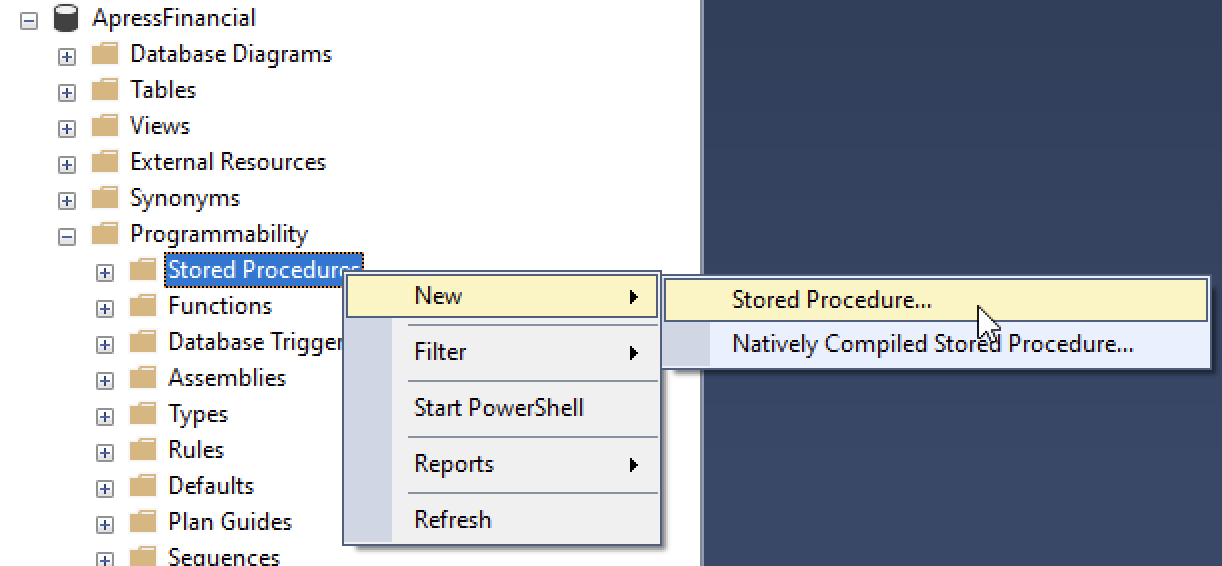
\includegraphics[width=0.6\textwidth]{images/task-1/1.png}
  \caption{Меню открытия окна создания хранимых процедур}
  \label{fig:task-1-1}
\end{figure}

\begin{figure}[H]
  \centering
  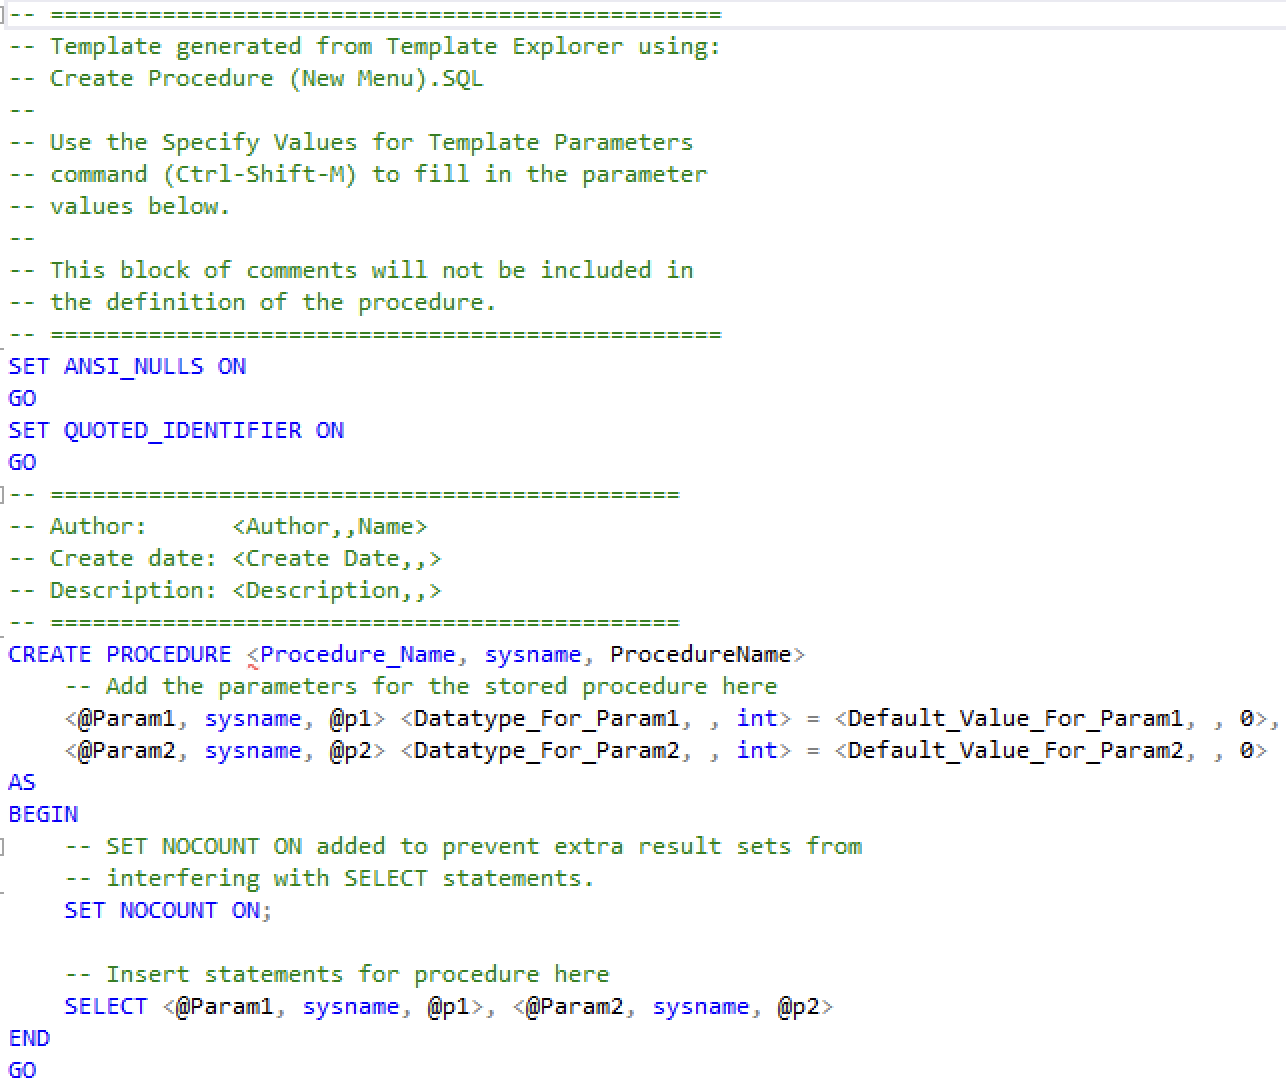
\includegraphics[width=0.9\textwidth]{images/task-1/2.png}
  \caption{Окно создания хранимой процедуры}
  \label{fig:task-1-2}
\end{figure}

\begin{figure}[H]
  \centering
  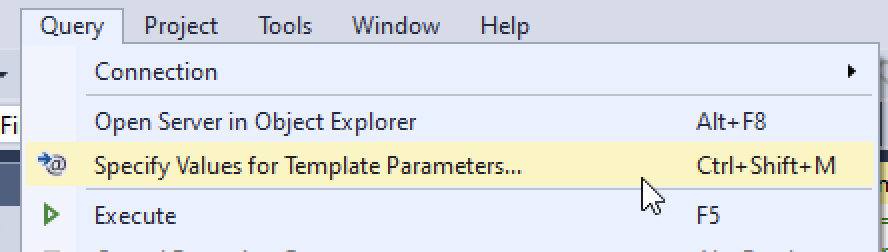
\includegraphics[width=0.5\textwidth]{images/task-1/3.png}
  \caption{Меню открытия окна настроек переменных шаблона}
  \label{fig:task-1-3}
\end{figure}

\begin{figure}[H]
  \centering
  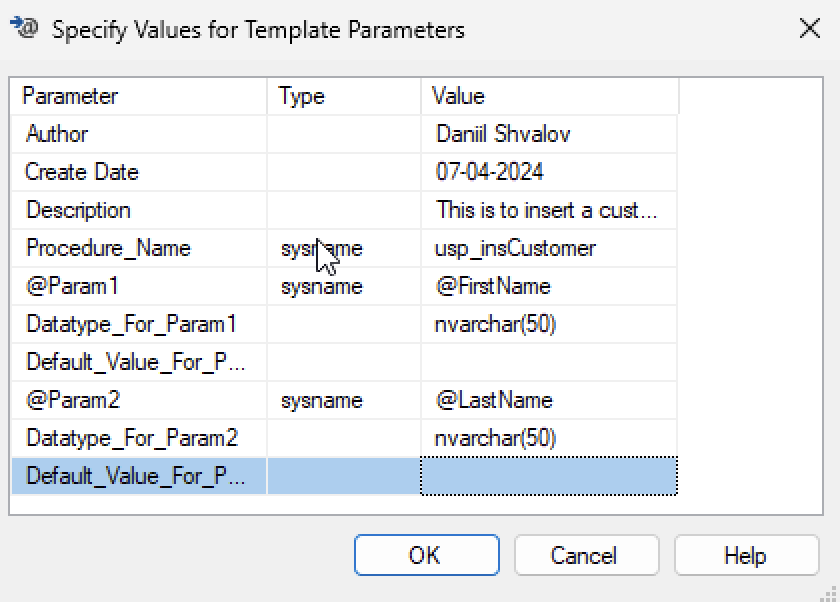
\includegraphics[width=0.7\textwidth]{images/task-1/4.png}
  \caption{Окно настроек переменных шаблона}
  \label{fig:task-1-4}
\end{figure}

\begin{figure}[H]
  \centering
  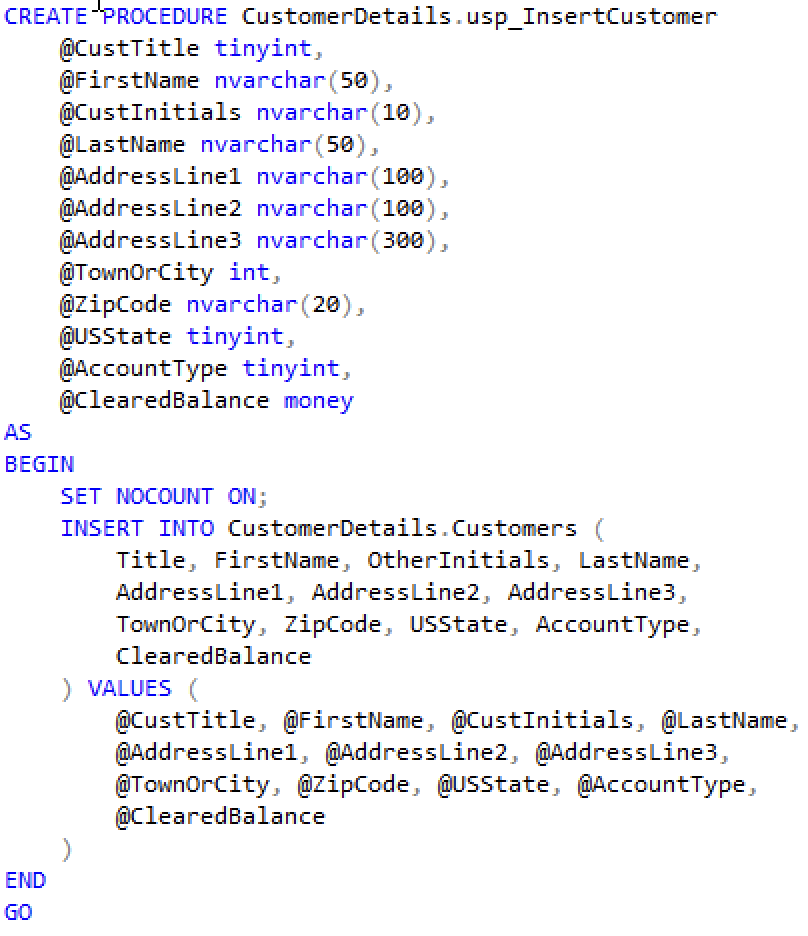
\includegraphics[width=0.7\textwidth]{images/task-1/5.png}
  \caption{
    Запрос для создания хранимой процедуры <<usp\_InsertCustomer>>
  }
  \label{fig:task-1-5}
\end{figure}

\begin{figure}[H]
  \centering
  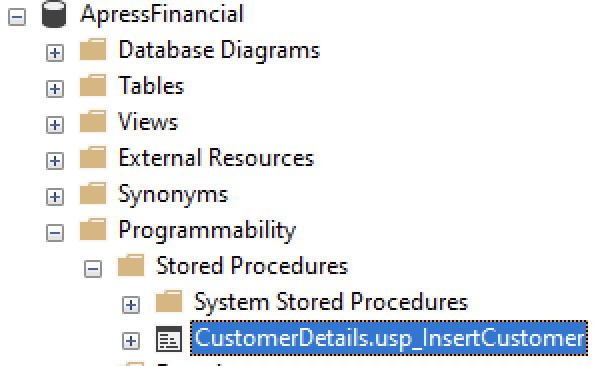
\includegraphics[width=0.5\textwidth]{images/task-1/6.png}
  \caption{Созданная процедура в интерфейсе SSMS}
  \label{fig:task-1-6}
\end{figure}

\subsubsection{Тестирование хранимой процедуры}

Для тестирования созданной процедуры был использован запрос, показанный на
рисунке \ref{fig:task-1-7}. С помощью данного запроса в таблицу
<<\foreignlanguage{english}{Customers}>> вставляются новые строки. С помощью
запроса, изображенном на рисунке \ref{fig:task-1-8}, были выведены созданные
процедурой строки. Как видно на рисунке \ref{fig:task-1-9}, новые строки
соответствуют ожидаемым.

\begin{figure}[H]
  \centering
  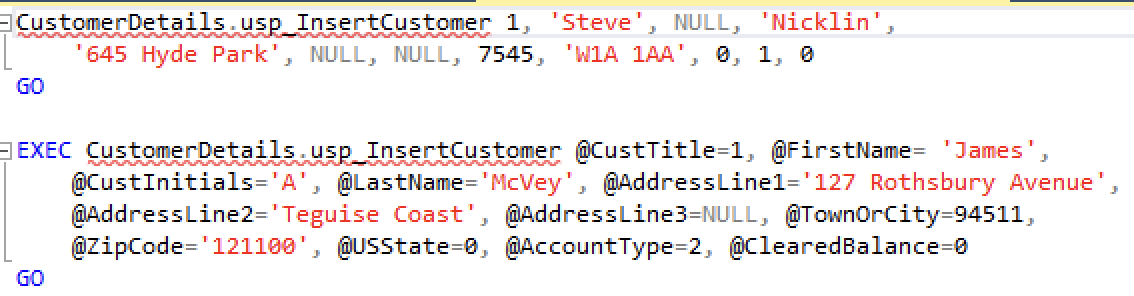
\includegraphics[width=\textwidth]{images/task-1/7.png}
  \caption{Вызов созданной процедуры}
  \label{fig:task-1-7}
\end{figure}

\begin{figure}[H]
  \centering
  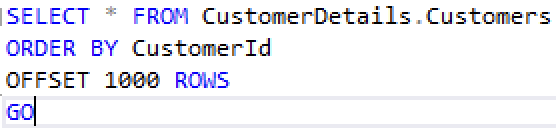
\includegraphics[width=0.6\textwidth]{images/task-1/8.png}
  \caption{Запрос для проверки работы процедуры}
  \label{fig:task-1-8}
\end{figure}

\begin{figure}[H]
  \centering
  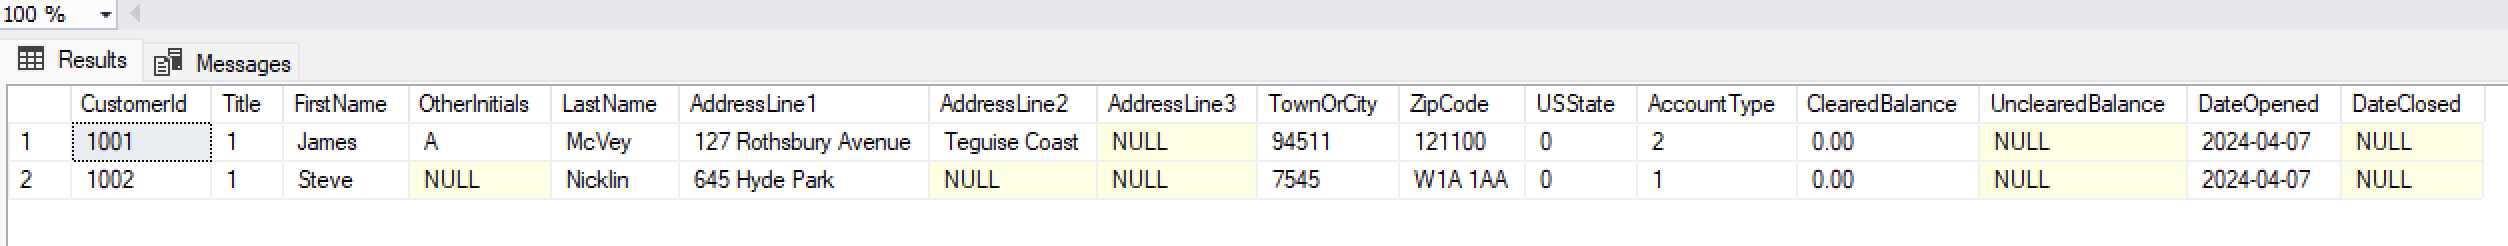
\includegraphics[width=\textwidth]{images/task-1/9.png}
  \caption{Созданные строки}
  \label{fig:task-1-9}
\end{figure}

\subsection{Вторая задача}

\subsubsection{Создание хранимой процедуры с помощью Query Editor}

С помощью запроса, показанного на рисунке \ref{fig:task-2-1}, была создана
процедура <<\foreignlanguage{english}{usp\_CustMovement}>>. После выполнения
данного запроса новая процедура появилась в интерфейсе SSMS (рисунок
\ref{fig:task-2-2}).

\begin{figure}[H]
  \centering
  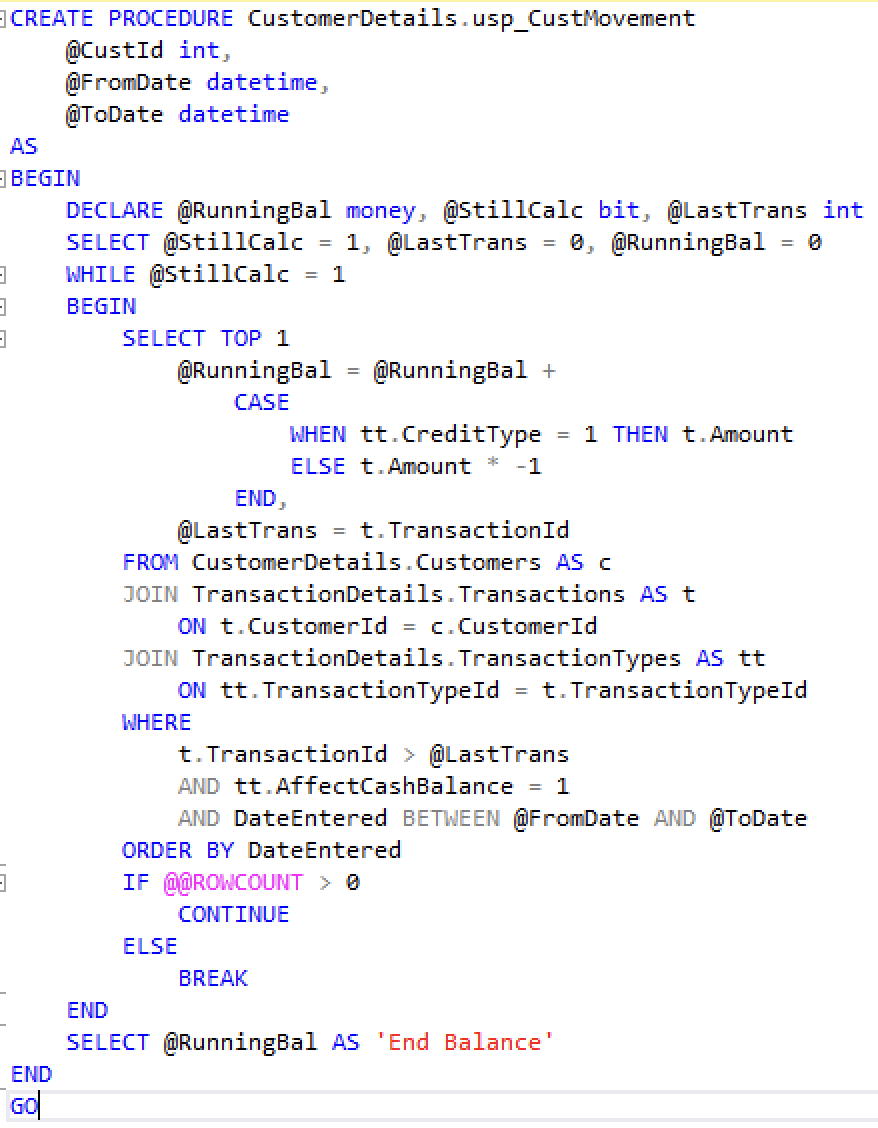
\includegraphics[width=0.8\textwidth]{images/task-2/1.png}
  \caption{
    Запрос для создания процедуры
    <<\foreignlanguage{english}{usp\_CustMovement}>>
  }
  \label{fig:task-2-1}
\end{figure}

\begin{figure}[H]
  \centering
  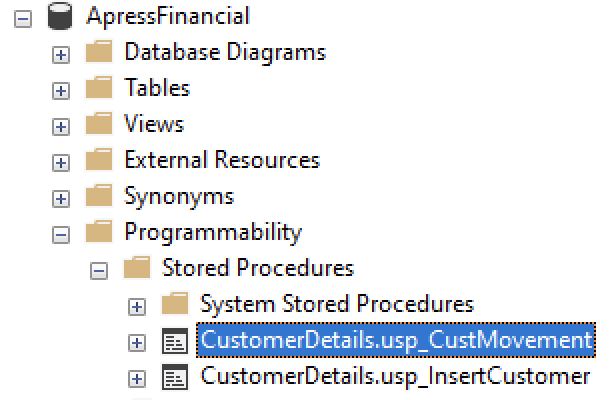
\includegraphics[width=0.5\textwidth]{images/task-2/2.png}
  \caption{Созданная процедура}
  \label{fig:task-2-2}
\end{figure}

\subsubsection{Тестирование хранимой процедуры}

С помощью запроса, показанного на рисунке \ref{fig:task-2-3}, были добавлены
тестовые данные в таблицу <<\foreignlanguage{english}{Transactions}>>. Затем, с
помощью запроса, изображенном на рисунке \ref{fig:task-2-4}, была вызвана
созданная хранимая процедура. Как видно на рисунке \ref{fig:task-2-5},
результат совпадает с ожидаемым.

\begin{figure}[H]
  \centering
  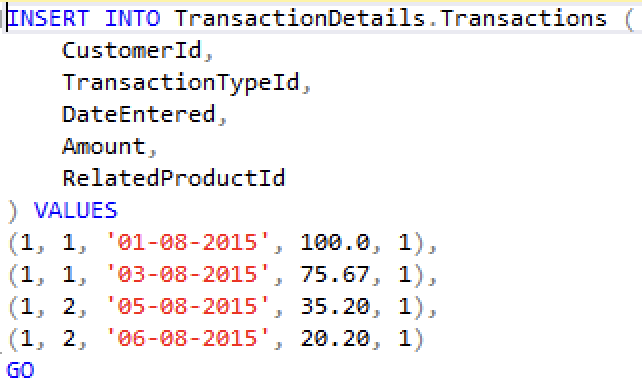
\includegraphics[width=0.8\textwidth]{images/task-2/3.png}
  \caption{Запрос для добавления тестовых данных}
  \label{fig:task-2-3}
\end{figure}

\begin{figure}[H]
  \centering
  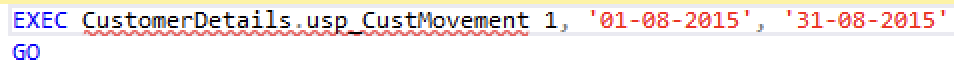
\includegraphics[width=\textwidth]{images/task-2/4.png}
  \caption{Запрос для вызова созданной процедуры}
  \label{fig:task-2-4}
\end{figure}

\begin{figure}[H]
  \centering
  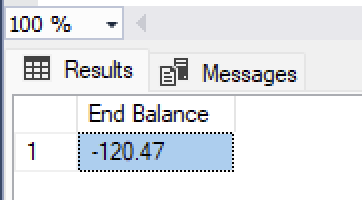
\includegraphics[width=0.4\textwidth]{images/task-2/5.png}
  \caption{Результат вызова процедуры}
  \label{fig:task-2-5}
\end{figure}

\subsection{Третья задача}

\subsubsection{Создание скалярной функции}

С помощью запроса, показанного на рисунке \ref{fig:task-3-1}, была создана
скалярная функция <<\foreignlanguage{english}{ufn\_IntCalc}>>, которая
рассчитывает сумму начислений на заданную сумму денежных средств за определенный
период времени. После выполнения данного запроса, новая функция появилась в
интерфейсе SSMS (рисунок \ref{fig:task-3-2}).

\begin{figure}[H]
  \centering
  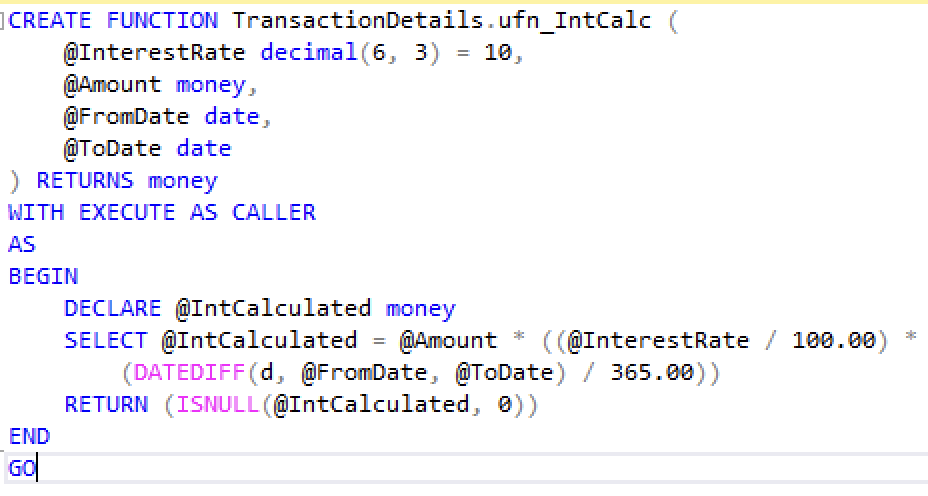
\includegraphics[width=\textwidth]{images/task-3/1.png}
  \caption{
    Запрос для создания скалярной функции
    <<\foreignlanguage{english}{ufn\_IntCalc}>>
  }
  \label{fig:task-3-1}
\end{figure}

\begin{figure}[H]
  \centering
  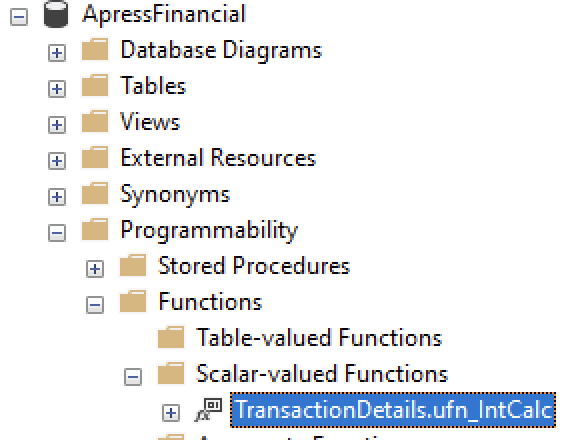
\includegraphics[width=0.6\textwidth]{images/task-3/2.png}
  \caption{Созданная процедура}
  \label{fig:task-3-2}
\end{figure}

\subsubsection{Тестирование функции}

С помощью запроса, показанного на рисунке \ref{fig:task-3-3}, была
протестирована созданная функция. Как видно на рисунке \ref{fig:task-3-4},
результат совпал с ожидаемым значением.

\begin{figure}[H]
  \centering
  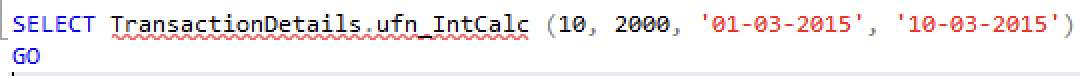
\includegraphics[width=\textwidth]{images/task-3/3.png}
  \caption{Запрос для тестирования созданной функции}
  \label{fig:task-3-3}
\end{figure}

\begin{figure}[H]
  \centering
  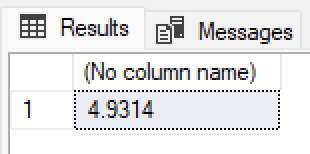
\includegraphics[width=0.4\textwidth]{images/task-3/4.png}
  \caption{Результат вызова функции}
  \label{fig:task-3-4}
\end{figure}

\subsection{Четвертая задача}

\subsubsection{Создание функции, возвращающей табличное значение}

С помощью запроса, показанного на рисунке \ref{fig:task-4-1}, была создана
функция, возвращающая информацию о транзакциях клиента. После выполнения данного
запроса новая функция появилась в интерфейсе SSMS (рисунок \ref{fig:task-4-2}).

\begin{figure}[H]
  \centering
  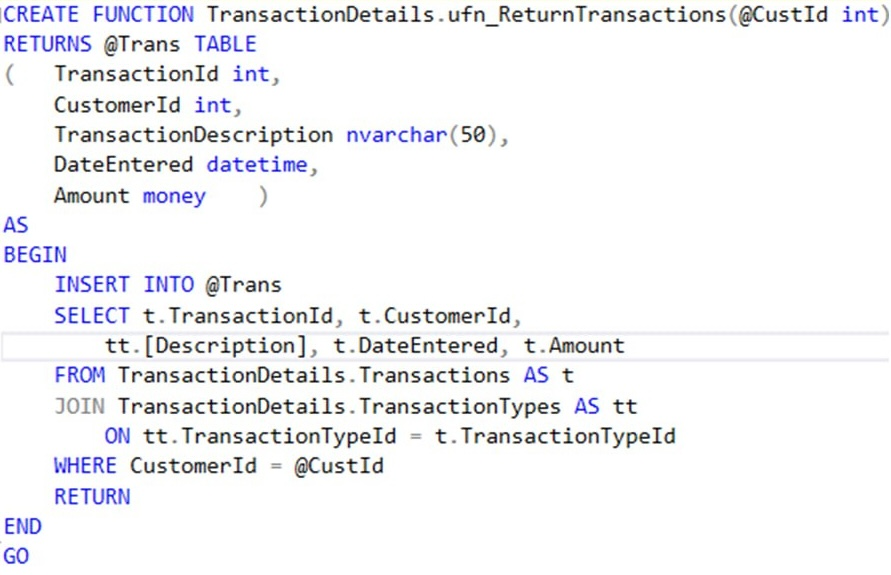
\includegraphics[width=\textwidth]{images/task-4/1.png}
  \caption{
    Запрос для создания функции
    <<\foreignlanguage{english}{ufn\_ReturnTransactions}>>, возвращающей
    табличное значение
  }
  \label{fig:task-4-1}
\end{figure}

\begin{figure}[H]
  \centering
  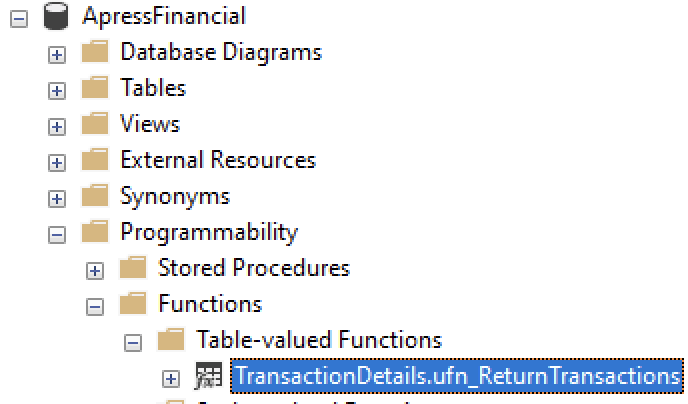
\includegraphics[width=0.6\textwidth]{images/task-4/2.png}
  \caption{Созданная функция}
  \label{fig:task-4-2}
\end{figure}

\subsubsection{Тестирование созданной функции}

С помощью запроса, показанного на рисунке \ref{fig:task-4-3}, была
протестирована новая функция. В данном есть два подзапроса: один использует
<<\foreignlanguage{english}{CROSS APPLY}>>, другой ---
<<\foreignlanguage{english}{OUTER APPLY}>>. Разница между этими методами в том,
что <<\foreignlanguage{english}{CROSS APPLY}>> возвращает только те строки,
которые есть как в таблице, так и в результате вызова функции, а
<<\foreignlanguage{english}{OUTER APPLY}>> возвращает строки, которые есть в
таблице, но необязательно есть в результате вызова функции. Как видно на рисунке
\ref{fig:task-4-4}, во втором случае есть строки с неопределенным значением.

\begin{figure}[H]
  \centering
  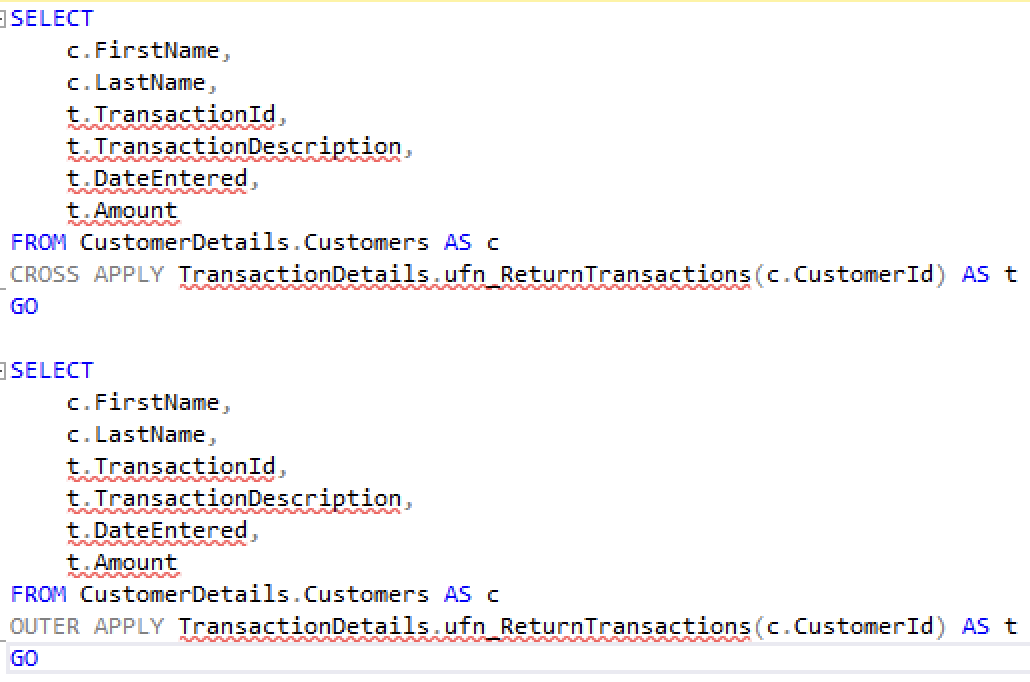
\includegraphics[width=\textwidth]{images/task-4/3.png}
  \caption{Запрос для тестирования созданной функции}
  \label{fig:task-4-3}
\end{figure}

\begin{figure}[H]
  \centering
  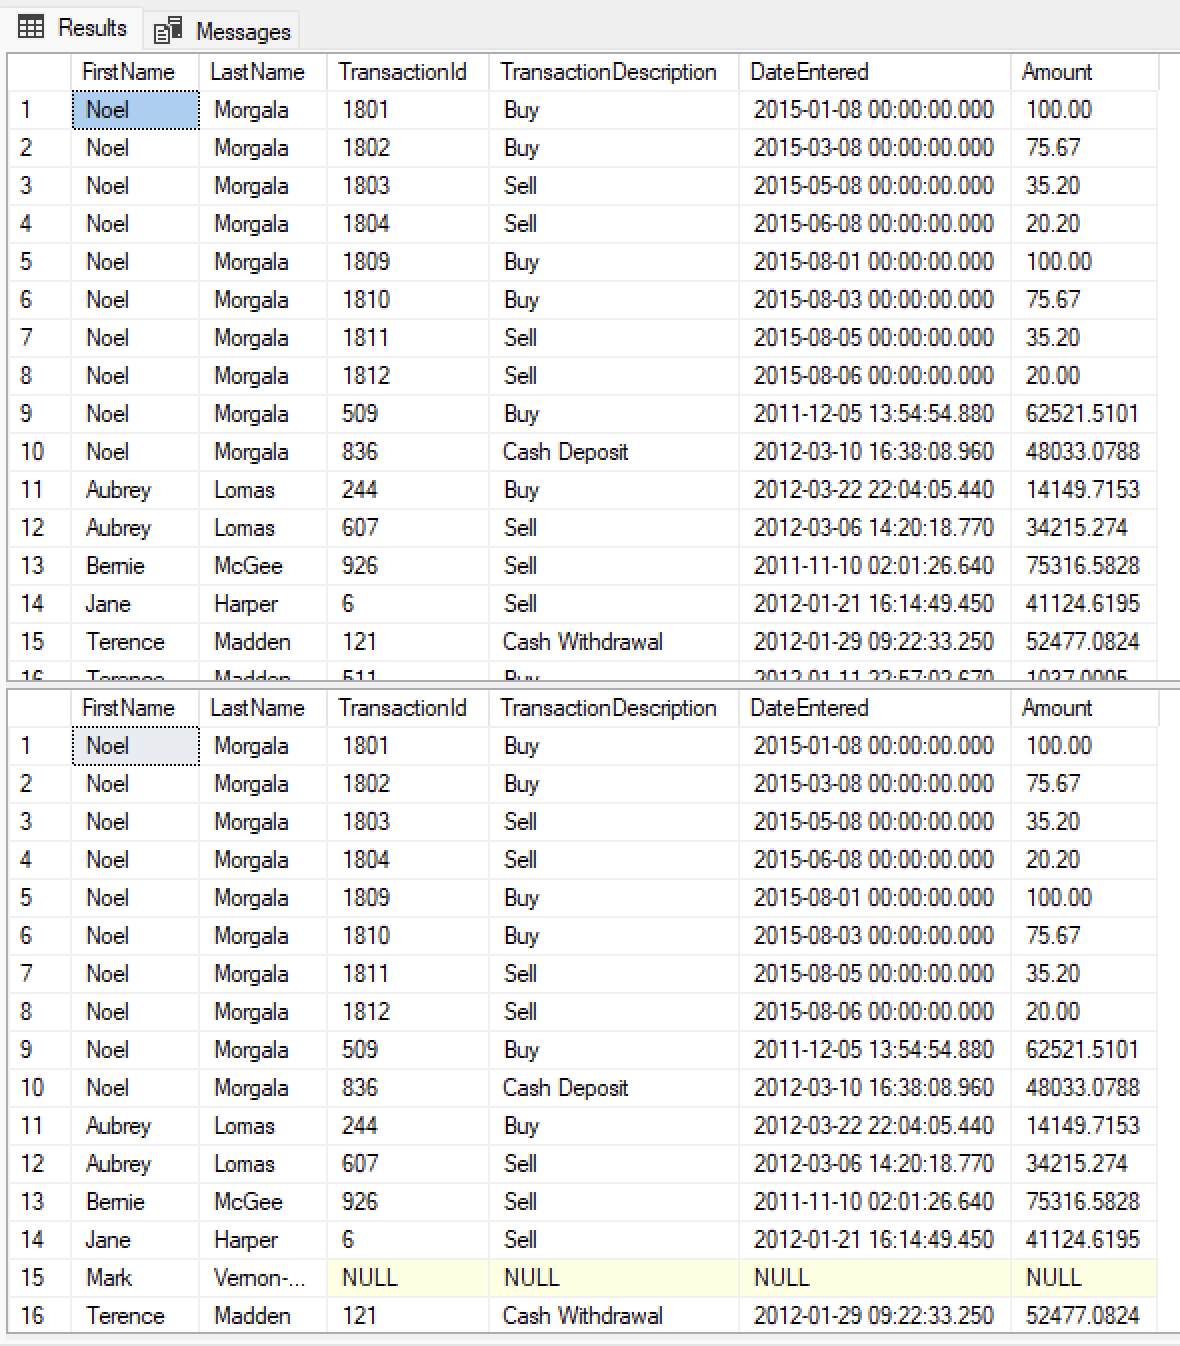
\includegraphics[width=\textwidth]{images/task-4/4.png}
  \caption{Результат выполнения запроса}
  \label{fig:task-4-4}
\end{figure}

\subsection{Пятая задача}

\subsubsection{Создание хранимой процедуры для вывода информации об акциях}

С помощью запроса, показанного на рисунке \ref{fig:task-5-1} была создана
процедура <<\foreignlanguage{english}{usp\_AllShareDetails}>>, которая принимает
ID акции и выводит для него:
\begin{itemize}
  \item выборку из таблицы Shares, содержащую ID акции, название и номер для
  фондового рынка;
  \item отсортированную выборку из таблицы SharePrices по дате цены в убывающем
  порядке, содержащую ID цены, ID акции, цену акции и дату этой цены.
\end{itemize}
В данной процедуре используется два запроса: первый выводит информацию об
определенной акции, а второй --- информацию о ценах данной акции. После
выполнения данного запроса процедура появилась в интерфейсе SSMS (рисунок
\ref{fig:task-5-2}).

При вызове данной процедуры, например, для ID акции, равной 1, выводятся
результаты, показанные на рисунке \ref{fig:task-5-3}.

\begin{figure}[H]
  \centering
  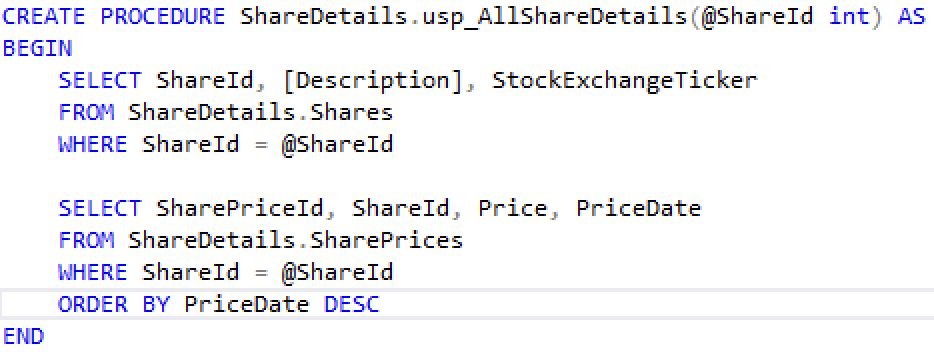
\includegraphics[width=\textwidth]{images/task-5/1.png}
  \caption{
    Запрос для создания процедуры
    <<\foreignlanguage{english}{usp\_AllShareDetails}>>
  }
  \label{fig:task-5-1}
\end{figure}

\begin{figure}[H]
  \centering
  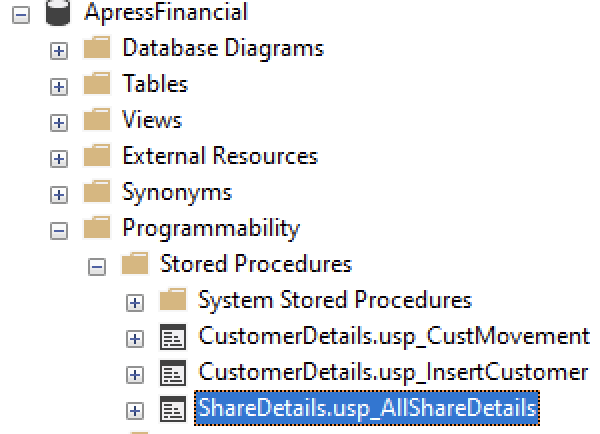
\includegraphics[width=0.6\textwidth]{images/task-5/2.png}
  \caption{Созданная процедура}
  \label{fig:task-5-2}
\end{figure}

\begin{figure}[H]
  \centering
  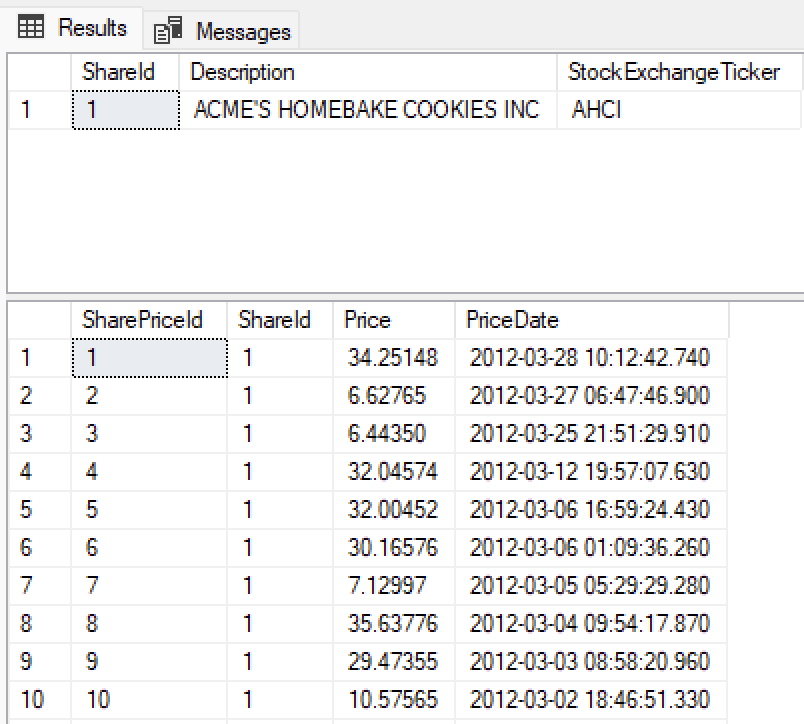
\includegraphics[width=0.8\textwidth]{images/task-5/3.png}
  \caption{Пример работы процедуры}
  \label{fig:task-5-3}
\end{figure}

\section{Выводы и анализ результатов работы}

В данной лабораторной работе изучены способы создания хранимых процедур и
функций в SSMS. В ходе выполнения лабораторной работы были созданы несколько
хранимых процедур и функций. Как было показано, процедуры и функции являются
очень полезным инструментом, позволяющим автоматизировать различные процессы при
работе с базой данных. При этом SSMS предоставляет различные способы, по-своему
удобные, для создания хранимых процедур и функций. Все это делает работу с
процедурами и функциями не только полезной, но и удобной.

Цель, поставленная в начале работы, достигнута, задачи выполнены.

\end{document}
